\section{Experiments and Results}
\label{sec:results}

We organize this section by research question. For each RQ we state the test, then report the result; full model specifications are in \autoref{sec:methods:stats}.

\paragraph{RQ1: a modest, directionally consistent uncertainty effect that does not survive multiple-comparison correction.}
For each model we split dialogues correct at $T_0$ by baseline entropy (\autoref{sec:methods:entropy}) into a certain group ($H=0$) and an uncertain group ($H<0$), and compare the rate of ever flipping across $T_1$--$T_6$ with a cluster bootstrap (resampling questions) for the gap's confidence interval and a cluster-robust logistic test, Holm-corrected across all 16 (model, dataset) cells.

\begin{table*}[t]
\centering
\caption{RQ1: Flip rates (\%) for certain ($H=0$) and uncertain ($H<0$) questions, restricted to dialogues correct at $T_0$ under the $R=3$ protocol. Pool denotes questions shared across models; $n_q^{T_0}$ counts questions with at least one correct initial response, and $n_{\text{dlg}}$ gives eligible dialogues (certain/uncertain). $\Delta$ is the flip-rate difference (uncertain $-$ certain, pp), with 95\% question-cluster bootstrap CIs (2,000 resamples). $p_{\text{Holm}}$ denotes one-sided cluster-robust logistic-test $p$-values, Holm-adjusted across 16 cells. \texttt{--} indicates missing groups or non-estimable tests due to perfect separation. $^\ddagger$ denotes a Newcombe (1998) hybrid-score CI used when identical ceiling rates yield a degenerate bootstrap CI.}
\label{tab:rq1}
\small
\begin{tabular}{llrrrrrcc}
\toprule
\textbf{Dataset} & \textbf{Model} & \textbf{Pool} & $n_q^{T_0}$ & $n_{\text{dlg}}$ (cert./unc.) & \textbf{Certain} & \textbf{Uncertain} & $\Delta$ [95\% CI] & $p_{\text{Holm}}$ \\
\midrule
MMLU-Pro & Claude Haiku & 420 & 349 & 671/277 & 89.9 & 95.3 & +5.4 [-0.2, +10.5] & 0.412 \\
MMLU-Pro & Claude Sonnet & 420 & 378 & 1014/85 & 70.8 & 83.5 & +12.7 [-1.4, +25.4] & 0.457 \\
MMLU-Pro & GPT-5.4 & 420 & 360 & 873/163 & 44.0 & 55.8 & +11.8 [-0.0, +23.3] & 0.261 \\
MMLU-Pro & GPT-5.4 Mini & 420 & 346 & 715/232 & 50.2 & 58.2 & +8.0 [-3.8, +18.7] & 0.500 \\
MMLU-Pro & GPT-5.4 Nano & 420 & 320 & 729/96 & 55.3 & 40.6 & -14.7 [-29.9, +1.3] & 1.000 \\
GPQA-Diamond & Claude Haiku & 198 & 152 & 165/208 & 98.2 & 100.0 & +1.8 [+0.0, +5.9] & -- \\
GPQA-Diamond & Claude Sonnet & 198 & 166 & 354/105 & 92.9 & 100.0 & +7.1 [+3.4, +11.0] & -- \\
GPQA-Diamond & GPT-5.4 & 198 & 171 & 366/90 & 67.5 & 68.9 & +1.4 [-14.8, +16.8] & 1.000 \\
GPQA-Diamond & GPT-5.4 Mini & 198 & 139 & 250/93 & 72.4 & 86.0 & +13.6 [-0.1, +26.2] & 0.412 \\
GPQA-Diamond & GPT-5.4 Nano & 198 & 146 & 260/65 & 59.2 & 44.6 & -14.6 [-32.8, +6.3] & 1.000 \\
HLE & Claude Haiku & 160 & 29 & 45/0 & 100.0 & -- & -- & -- \\
HLE & Claude Sonnet & 160 & 48 & 76/27 & 97.4 & 100.0 & +2.6 [+0.0, +9.4] & -- \\
HLE & GPT-5.4 & 160 & 40 & 53/25 & 88.7 & 96.0 & +7.3 [-4.8, +20.8] & 0.641 \\
HLE & GPT-5.4 Mini & 160 & 28 & 34/14 & 94.1 & 100.0 & +5.9 [+0.0, +18.2] & -- \\
HLE & GPT-5.4 Nano & 160 & 35 & 37/10 & 100.0 & 100.0 & +0.0 [-27.8, +9.4]$^\ddagger$ & -- \\
HLE & Gemini 3.5 Flash & 160 & 80 & 105/96 & 66.7 & 77.1 & +10.4 [-6.1, +27.0] & 0.556 \\
\bottomrule
\end{tabular}

\footnotesize \texttt{Reproducibility: analysis/paper\_pipeline.py}
\end{table*}

On MMLU-Pro, four of five models show the expected direction (uncertain flips more than certain), from $+5.4$pp (Claude Haiku) to $+12.7$pp (Claude Sonnet); GPT-5.4 Nano reverses ($-14.7$pp). None survive Holm correction (smallest $p_{\text{Holm}}=0.261$). On GPQA-Diamond, Claude Sonnet shows a real effect once GPQA gaps are filled: $92.9\%$ certain vs.\ $100.0\%$ uncertain, bootstrap CI $[+3.4,+11.0]$ excluding zero -- though the uncertain group's $100\%$ ceiling means the logistic test's $p$-value is not estimable there. The other GPQA models are mixed and not individually significant. HLE samples are small (Claude Haiku has no uncertain-group questions at all; other cells range $n=28$--$80$) and mostly near ceiling, so we read HLE as underpowered for this contrast rather than as evidence against the effect.

\paragraph{RQ2: pressure and uncertainty each predict flipping on their own; their interaction does not.}
\label{sec:exp2}
For each (model, dataset) condition we fit flip outcome on pressure level $P$, mean-centered entropy $H_c$, and their interaction $P H_c$ (\autoref{sec:methods:stats}).

\begin{figure*}[t]
\centering
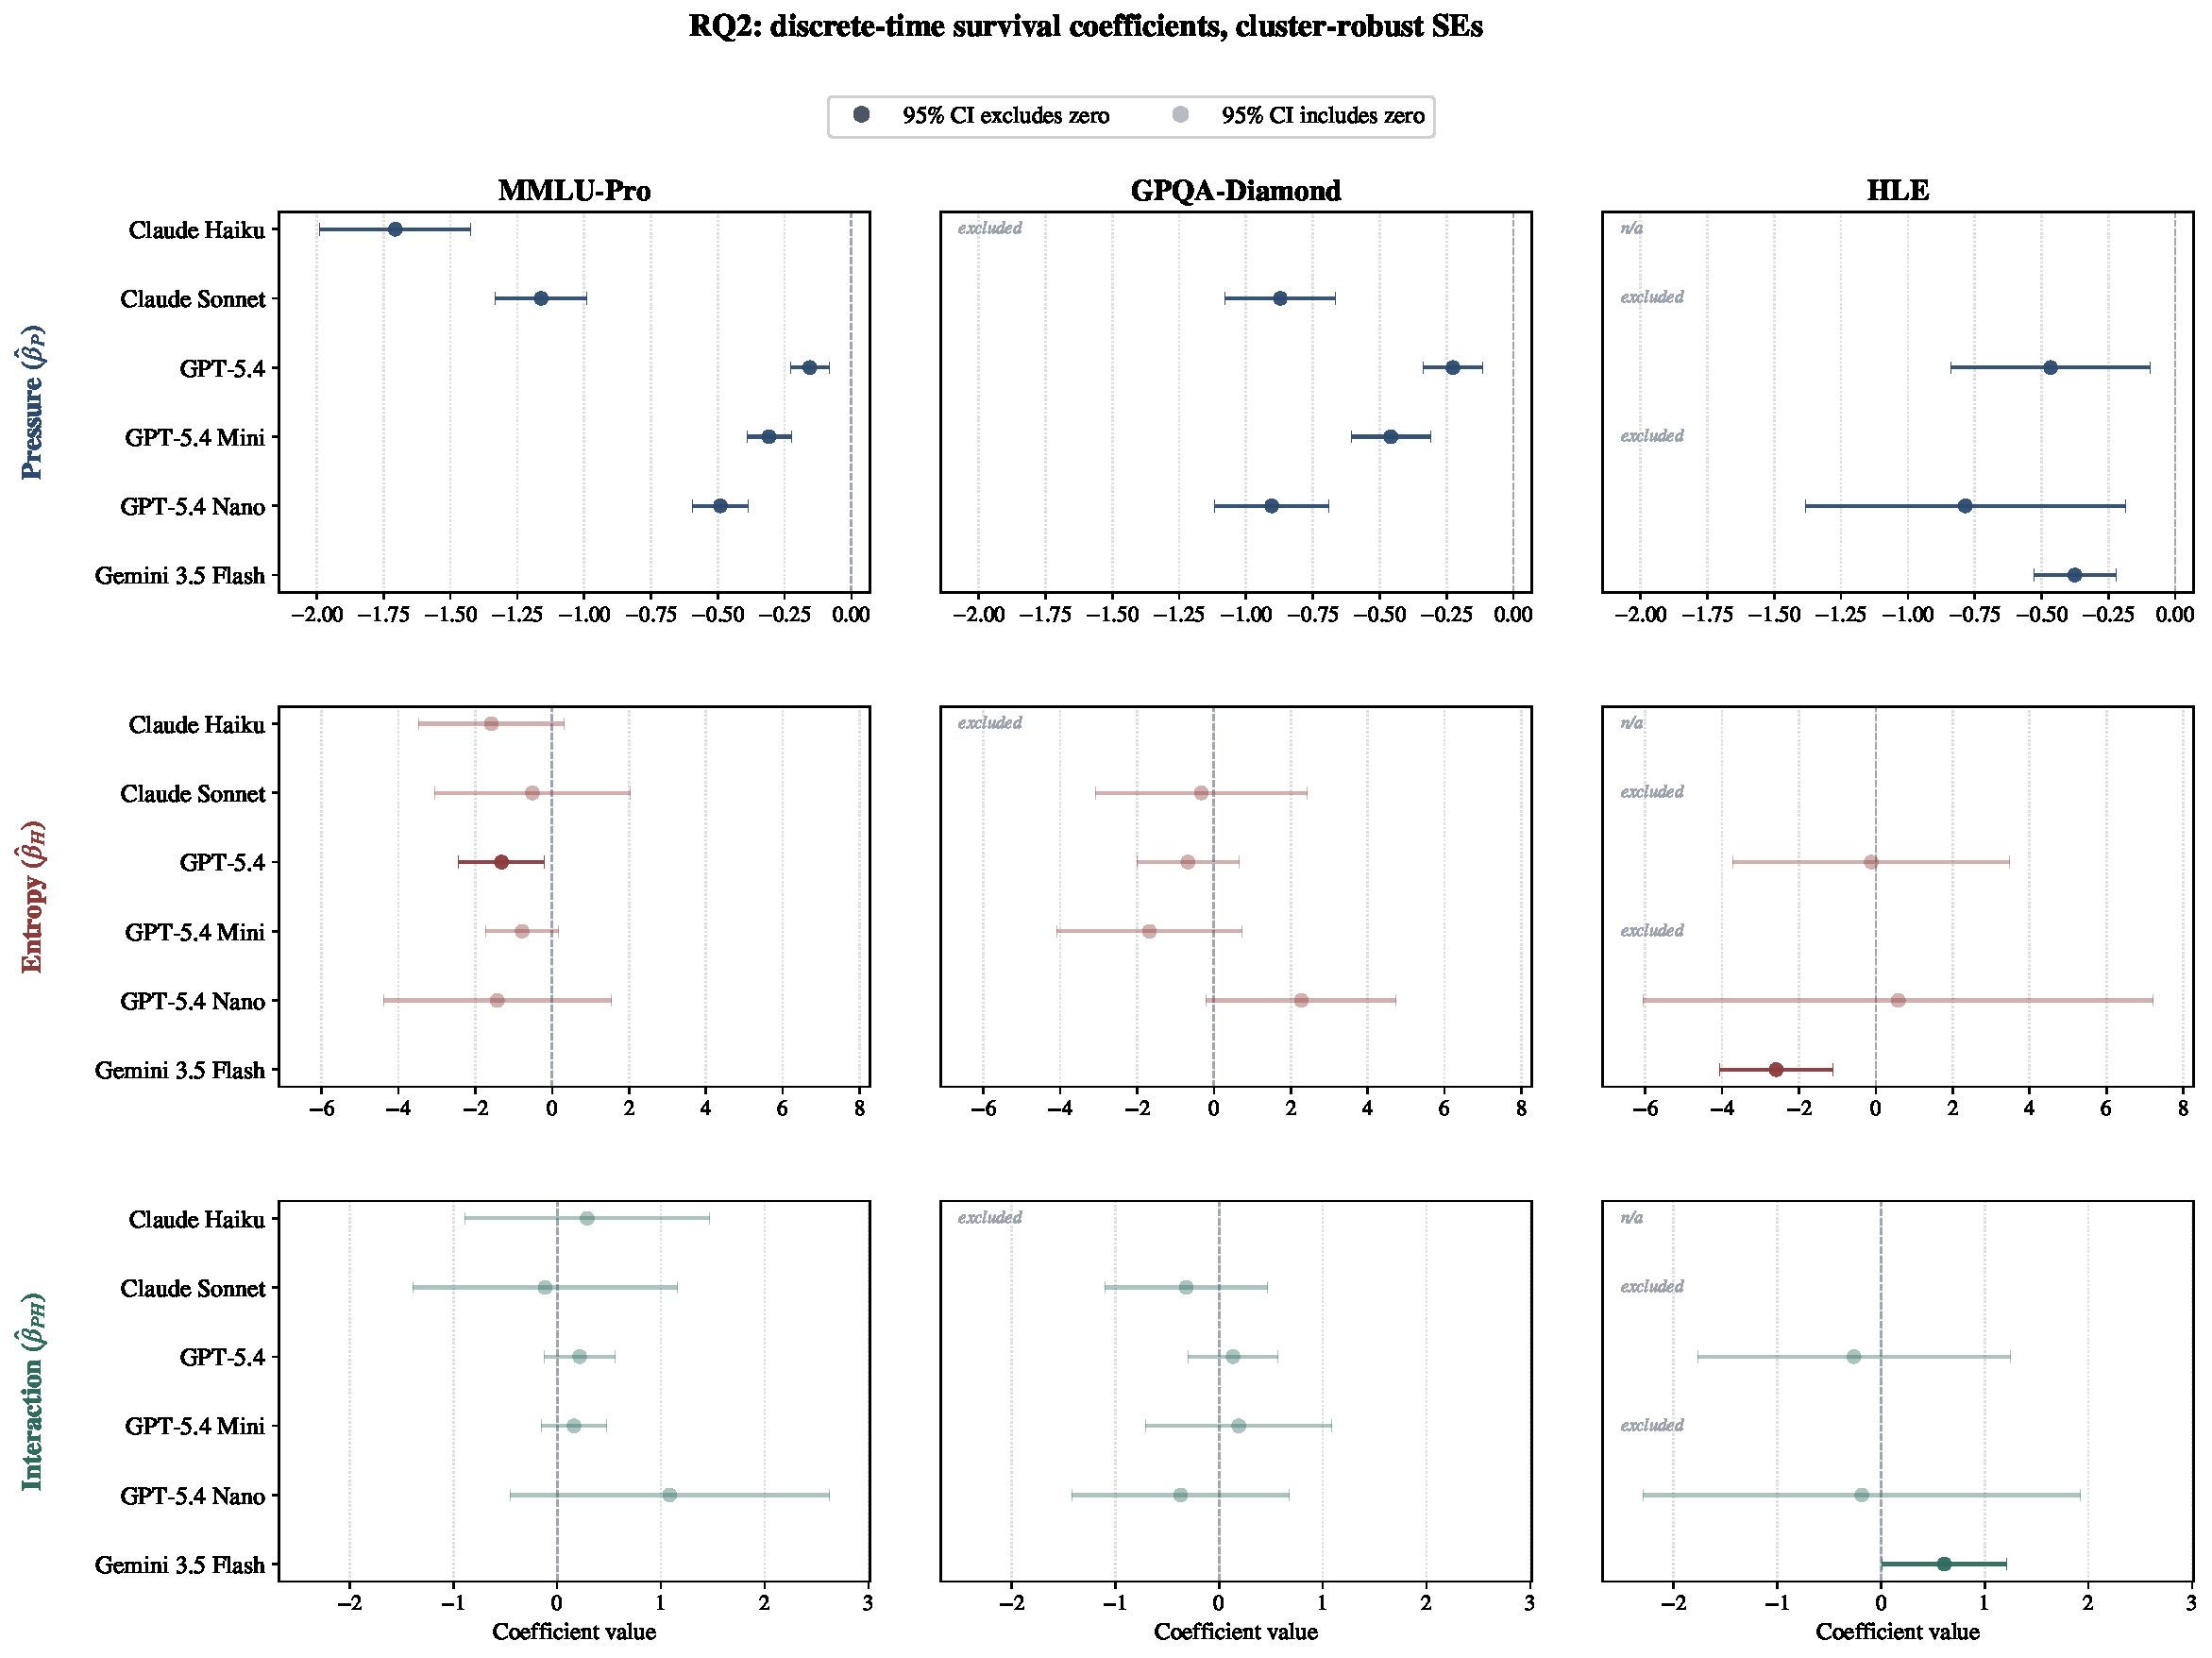
\includegraphics[width=\textwidth]{sections/fig/rq2_coefs.pdf}
\caption{RQ2: discrete-time survival coefficients with cluster-robust 95\% CIs, by (model, dataset). $\hat\beta_P$ sign splits models into resisters (negative) and capitulators (positive), significant in every identifiable condition. $\hat\beta_H$ is directionally mixed and individually significant only for GPT-5.4 on MMLU-Pro. $\hat\beta_{PH}$ (faded where its CI includes zero) is significant in only one cell, Gemini 3.5 Flash on HLE; separation-flagged cells are omitted. Full values in \autoref{app:rq2_table}.}
\label{fig:rq2_coefs}
\end{figure*}

$\hat\beta_P$ splits models into resisters (Claude Haiku, Claude Sonnet, GPT-5.4) and capitulators (GPT-5.4 Mini, Nano), consistently significant in every identifiable condition. $\hat\beta_H$ is directionally mixed on MMLU-Pro and individually significant for only GPT-5.4; the near-ceiling flip rates in several cells make its magnitude uninformative even where its sign is. The interaction $\hat\beta_{PH}$ is \emph{not} individually significant in any of the five MMLU-Pro conditions (all $p>0.1$; full values in \autoref{app:rq2_table}): Claude Sonnet's own estimate is $-0.117$ ($p=0.86$).

Pooling the per-model $\hat\beta_{PH}$ estimates with a random-effects meta-analysis \citep{dersimonian1986meta} gives $+0.200$ on MMLU-Pro ($k=5$, all identifiable; $95\%$ CI $[-0.019,+0.419]$, $p=0.073$), $+0.029$ on GPQA-Diamond ($k=4$, Claude Haiku excluded for near-perfect separation; $95\%$ CI $[-0.305,+0.363]$, $p=0.864$), and $+0.448$ on HLE ($k=3$: GPT-5.4, GPT-5.4 Nano, and Gemini 3.5 Flash; Claude Haiku, Claude Sonnet, and GPT-5.4 Mini excluded for separation or lack of flip variance; $95\%$ CI $[-0.089,+0.985]$, $p=0.102$). None of the three pooled intervals excludes zero at $p<0.05$, so we report RQ2 as inconclusive rather than as a positive finding: pressure and uncertainty each predict flipping on their own, but we do not have reliable evidence that they interact.

\paragraph{RQ3: models split into resisters and capitulators, and the split breaks down on HLE.}
\label{sec:exp3}
We fit a mixed-effects extension of the RQ2 model with a model-level random intercept, and a model-agnostic linear trend on each model's per-turn flip rate across $T_1$--$T_6$, which ignores entropy and asks whether susceptibility rises or falls under sustained pressure. A high negative slope defines a \textbf{resister}, a high positive slope a \textbf{capitulator}.

Exact per-model slopes, significance tests, and behavioral
classifications are reported in \autoref{app:rq3_slopes}.
\begin{figure*}[t]
\centering
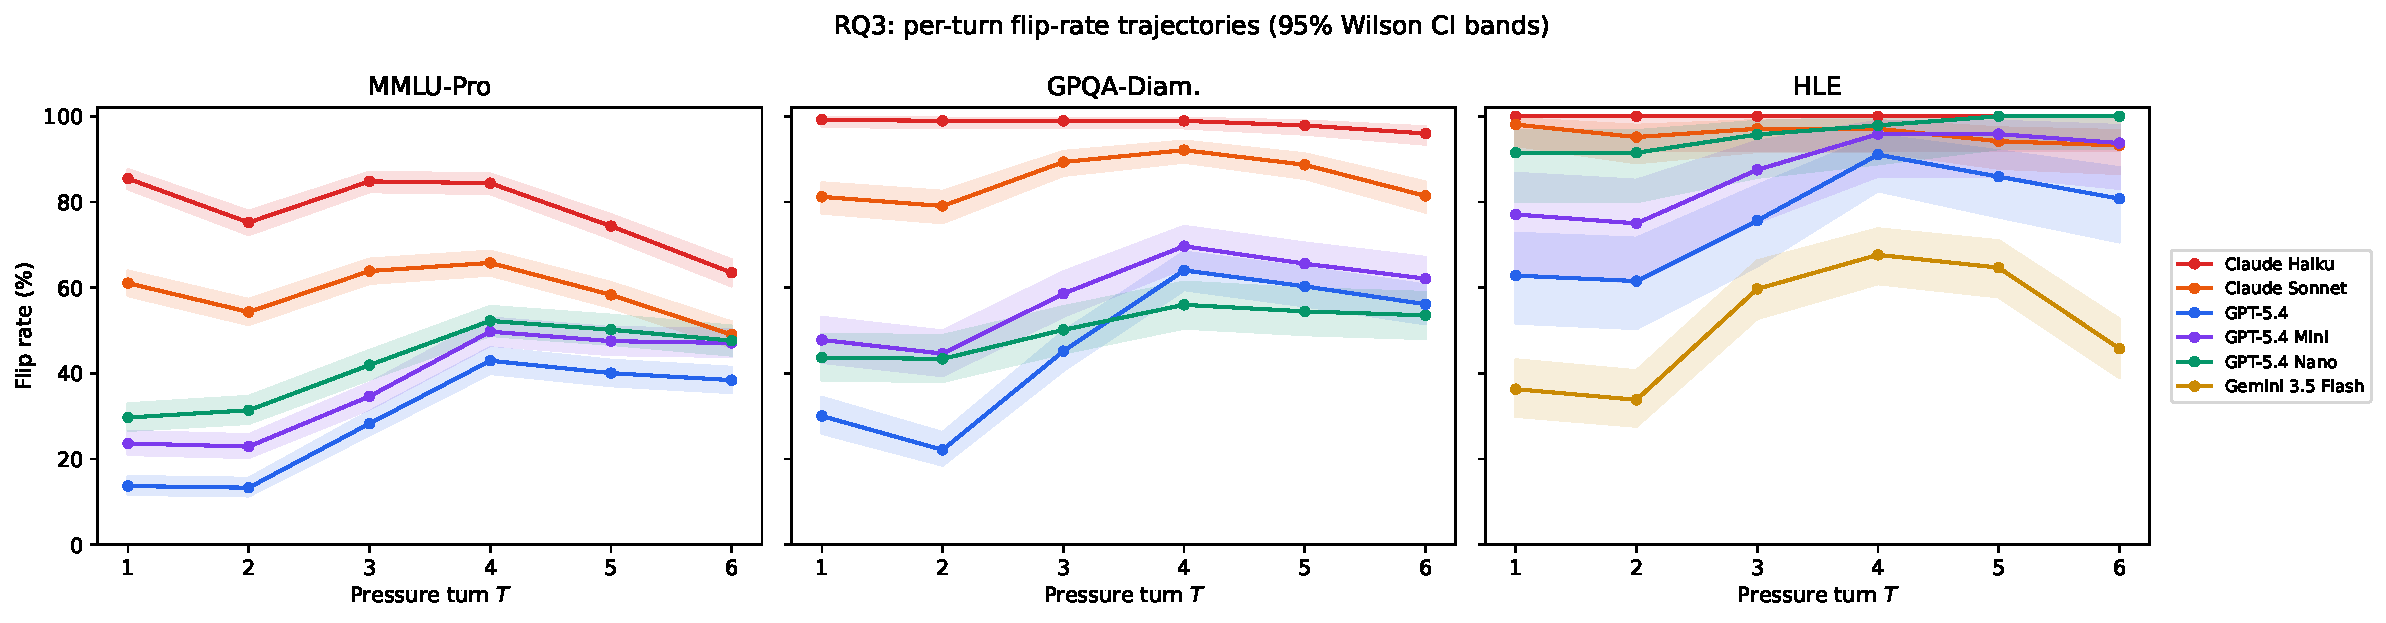
\includegraphics[width=\textwidth]{sections/fig/rq3_combined.pdf}
\caption{RQ3: per-turn flip-rate trajectories for each model. Shaded bands: 95\% Wilson CIs. On MMLU-Pro, Claude Haiku, Claude Sonnet, and GPT-5.4 decline (resist) while GPT-5.4 Mini and Nano grow (capitulate); on GPQA-Diamond and HLE, Claude Sonnet joins the capitulators (\autoref{tab:rq3}).}
\label{fig:rq3combined}
\end{figure*}

On MMLU-Pro, Claude Haiku, Claude Sonnet, and GPT-5.4 are resisters and GPT-5.4 Mini and Nano are capitulators, all individually significant (\autoref{fig:rq3combined}, \autoref{tab:rq3}). On GPQA-Diamond the same split holds for four of five models, but Claude Sonnet now capitulates (AME $+0.87$pp/turn, $p=0.012$) rather than resisting, the opposite of its MMLU-Pro behavior; Claude Haiku is flat (not significant). On HLE, Claude Haiku cannot be fit at all: it is wrong at every turn with no variance for a trend. Claude Sonnet is flat and slightly negative on HLE ($p=0.20$): no reliable trend in either direction. GPT-5.4, GPT-5.4 Mini, GPT-5.4 Nano, and Gemini 3.5 Flash all capitulate on HLE, each individually significant. The resister/capitulator label is therefore a property of a (model, benchmark-difficulty) pair, not a fixed model trait: GPT-5.4 resists on MMLU-Pro and GPQA-Diamond but capitulates on HLE, and Claude Sonnet resists on MMLU-Pro but capitulates on GPQA-Diamond.

\paragraph{Fragmentation is rare for Claude, modest for GPT, and substantial only for Gemini on HLE.} A query loses consensus at turn $t$ (\autoref{sec:methods:signals}) when no answer wins a majority across the $R=3$ canonical CoT dialogues (\autoref{sec:methods:stats}), among queries with a correct majority at $T_0$. Claude Haiku ($n=13$) and Claude Sonnet ($n=33$) lose consensus on $0\%$ of eligible queries (Wilson $95\%$ CI up to $22.8\%$ and $10.4\%$ respectively, reflecting the small $n$ rather than a precise zero), GPT-5.4 Mini $11.8\%$ $[3.3,34.3]$ and GPT-5.4 $16.7\%$ $[6.7,35.9]$, GPT-5.4 Nano $0\%$ $[0.0,27.8]$, and only Gemini 3.5 Flash shows fragmentation as a near-majority outcome at $45.5\%$ $[34.0,57.4]$ (\autoref{tab:rq4_hle}). A looser eligibility criterion (any dialogue, not a majority, correct at $T_0$; larger $n$ throughout) gives the same pattern within a few points, so this is not an artifact of the eligibility choice. Fragmentation remains a minor failure mode on MMLU-Pro and GPQA-Diamond for every model ($\leq 3.5\%$, \autoref{app:fragmentation}). \autoref{app:fragmentation} tests whether fragmentation risk reduces to each question's own baseline uncertainty rather than benchmark identity: the overall conclusion is that benchmark difficulty, not a clean per-question uncertainty gradient, dominates. What the RQ4 results below show directly is that Claude's actual HLE failure mode is not fragmentation but severe overconfidence: both Claude models' answers are highly consistent across dialogues even as they become near-certainly wrong and increasingly confident in that wrong answer.

\paragraph{RQ4: belief collapses at $T_1$, expressed confidence does not follow.}
Using the confidence estimator $\mathcal{C}$ (\autoref{sec:methods:calibrator}), we compute at each turn: belief entropy over run-level majority beliefs, majority-belief correctness, and mean confidence at the final reasoning step, giving the gap $\mathrm{Gap}_t$ (Conf.\ $-$ Maj.\ Correct). \autoref{fig:rq4combined} (\autoref{app:rq4}) plots the full $T_0$--$T_6$ trajectory.

Across all five Claude/GPT models on MMLU-Pro and GPQA-Diamond, majority correctness drops $31$--$65$ pp from $T_0$ to $T_6$ while mean confidence stays within $\pm10$ pp of its $T_0$ value in every condition and does not fall in step with correctness in any of them; the gap widens throughout because confidence does not track the correctness drop. Claude Haiku on GPQA-Diamond shows the largest gap: correctness falls from $0.646$ to $0.025$ while confidence rises from $0.830$ to $0.929$, a trajectory already substantial by $T_2$. On HLE, where only Claude and GPT-5.4 variants have a measurable majority at $T_0$, the same pattern is more extreme still: Claude Haiku's correctness falls from $0.087$ to $0.000$ while confidence rises from $0.796$ to $0.945$, and Claude Sonnet's from $0.234$ to $0.020$ while confidence rises from $0.806$ to $0.938$ (\autoref{tab:rq4_hle}) -- the two largest gaps in the study. Belief entropy tracks the same trend, so the estimator's read of the trace grows less stable under pressure even as expressed confidence does not move. An ensemble-level ECE check confirms the same dissociation and rules out a purely per-step artifact (\autoref{fig:ensemble_ece}, \autoref{app:calibration}).

\paragraph{Single-turn robustness.}
A single-turn MMLU-Pro experiment supports both the uncertainty effect (Spearman correlation between baseline entropy and flip rate, significant for three of six models) and the pressure-category ordering without multi-turn accumulation; full results are in \autoref{app:single_turn}.

% \paragraph{Single-turn robustness check.}
% To rule out that the RQ1 effect and the RQ3 ordering are artifacts of multi-turn accumulation, we ran a single-turn variant on MMLU-Pro: one pressure prompt after the baseline answer, per (model, question, category) cell (\autoref{tab:single_turn}). Both effects persist. The category ordering holds across all six models: expert authority is strongest, personal certainty and crowd consensus are consistently weakest (\autoref{app:single_turn}). The RQ1 gap also persists: uncertain-baseline questions flip $30$--$80\%$ more often than certain ones, with Spearman $\rho$ between baseline entropy and single-turn flip rate in $[-0.39,-0.05]$ per model (significant for three of six). Uncertainty conditioning reflects how a model responds to pressure in general.
